\newpage
\appendix
\section{Verificarlo-CI tutorial}
This tutorial for the CI functionality of Verificarlo is available as a
dedicated
repository\footnote{\url{https://github.com/verificarlo/vfc_ci_tutorial}}.
It describes how to setup the CI pipeline and generate the report on a simple
example.  Users can set up a CI workflow on the simple code transcribed here.

\begin{minted}{C}
#include <stdio.h>
#include <stdlib.h>
#include <time.h>
#define N 4096

float naiveDotprod(float * x, float * y, size_t n) {
	float res = 0;
	for(size_t i=0; i<n; i++) {
		res += x[i] * y[i];
	}
	return res;
}

int main(void) {
	float x, y [N];
	srand(42);
	for(size_t i=0; i<N; i++) {
		x[i] = (float) rand() / RAND_MAX;
		y[i] = (float) rand() / RAND_MAX;
	}
	srand(time(NULL));

	float naiveRes = naiveDotprod(x, y, N);
	printf("Naive dotprod = %.7f \n", naiveRes);

	return 0;
}
\end{minted}

The goal of this example is to compute a basic dot product on two vectors
generated with a fixed with random seed. The computation is done with a naive
method, and the function that does it can be found at the beginning of \texttt{main.c}.
The goal will be to use Verificarlo CI to measure the numerical accuracy of the
naive implementation, before adding a better version of the algorithm and
validating it by comparing the results of the two versions.

Following this tutorial will require you to have a functional install of
Verificarlo on your machine, or to use it through its Docker image. For more
information on the tool itself, please refer to the Verificarlo CI
documentation. It is advised that you at least go through it quickly before
doing this tutorial.

\subsection{Fork and clone the repository}

In order to follow this tutorial, which makes use of GitHub Actions, you will
need to have your own fork of this repository. Once it is created,
\mintinline{bash}{git clone} it:


\begin{minted}{bash}
$ git clone https://github.com/[YourUserName]/verificarlo_ci_tutorial
$ cd verificarlo_ci_tutorial
\end{minted}

\subsection{Try to build and execute the code}

Here is the output that you should get after issuing the following commands:

\begin{minted}{text}
$ make
$ ./dotprod
Naive dotprod = 1040.9039307
\end{minted}

\subsection{Add your first test probes}

\mintinline{C}{vfc_probes} is the system used by Verificarlo CI to export test variables from a program to the tool itself. First of all, you'll need to modify the Makefile to link the \mintinline{C}{vfc_probes} library. Line 4 should become:

\begin{minted}{make}
all:
	$(CC) main.c -lvfc_probes -o dotprod
\end{minted}

Moreover, you must also include the \mintinline{C}{vfc_probes.h} header at the
beginning of \mintinline{C}{main.c}. You should add the following include
statement after line 3:

\begin{minted}{C}
#include <vfc_probes.h>
\end{minted}

Now that \mintinline{C}{vfc_probes} is correctly linked, we can create out probes structure. This should be done at the beginning at the main function, for instance after the new line 20 (if you added the previous line):

\begin{minted}{C}
int main(void) {
  vfc_probes probes = vfc_init_probes();
\end{minted}

Then we will add the probe containing the result of the \texttt{dotprod}. You can do this after the new line 32:

\begin{minted}{C}
  float naiveRes = naiveDotprod(x, y, n);
  vfc_probe(&probes, "dotprod_test", "naive", naiveRes);
\end{minted}

Finally, we can dump the probes at the end of the main function, just before the return statement:

\begin{minted}{C}
  vfc_dump_probes(&probes);
  return 0;
\end{minted}


\subsection{Set up \texttt{vfc\_ci} and GitHub Actions}

Before setting up GitHub Actions, we need to make sure that the \mintinline{bash}{vfc_ci} test command can run. To do this, create \mintinline{bash}{vfc_tests_config.json}, the test configuration file, at the root of the repository and with the following content:

\begin{minted}{Python}
{
    "make_command": "make CC=verificarlo-c",
    "executables": [
        {
            "executable": "dotprod",
            "vfc_backends": [
                {
                    "name": "libinterflop_mca.so",
                    "repetitions": 20
                },
                {
                    "name": "libinterflop_mca.so --mode=rr",
                    "repetitions": 20
                }
            ]
        }
    ]
}
\end{minted}

Each test run will consist of 40 executions of the dotprod executable, split over two backends. This will export one test probe containing the result of the naive dotprod. To make sure that everything works correctly, it is possible to call \mintinline{bash}{vfc_ci} test with the dry run flag, so that no output file will be produced:

\begin{minted}{bash}
$ vfc_ci test -d
[...]
Info [vfc_ci]: The results have been successfully written to XXXXXXXXXX.vfcrun.h5.
Info [vfc_ci]: The dry run flag was enabled, so no files were actually created.
\end{minted}

If you get the following output, your Verificarlo CI setup should be correct.

Before setting up the CI workflow, we need to make sure that our local repository doesn't contain any unstaged changes. Commit and push the changes that you have just made:

\begin{minted}{bash}
$ git add .
$ git commit
$ git push --set-upstream origin master
\end{minted}

You are finally ready to create the CI workflow. This can be done automatically with the following command:

\begin{minted}{bash}
$ vfc_ci setup github
Info [vfc_ci]: A Verificarlo CI workflow has been setup on master.
Info [vfc_ci]: Make sure that you have a "vfc_tests_config.json" on this branch.
You can also perform a "vfc_ci test" dry run before pushing other commits.
\end{minted}

This should create a commit on the master branch (which we will call the dev
branch), as well as a \mintinline{bash}{vfc_ci_master} branch (which we will call the
CI branch). A first test run will also be triggered immediately after the
commit, which will result in a test file being committed to the CI branch.


\subsection{Serve the test report}

Once the test file has been committed to the CI branch, you can checkout to it and access the results:

\begin{minted}{bash}
$ git checkout vfc_ci master
$ git pull origin vfc_ci_master
$ cd vfcruns
$ vfc_ci test -s
\end{minted}

\dots will open the report in your browser.

There's not much to see for now, since there's only one test variable and one
run in the report. However, if the naive algorithm could seem sufficient at
first glance, it does have one issue. The values of \mintinline{C}{x[i] * y[i]}
are all added to the same \mintinline{C}{res} variable, which will suffer from increasingly
important round off errors. Thus, when a cancellation occurs, it will become
catastrophic and yield an inaccurate result. It has been shown that this error
grows in $O(n)$.


\subsection{Adding an improved method}

This subsection introduces another method for the computation of a dot product.
The idea is to recursively split the \mintinline{C}{x} and \mintinline{C}{y}
arrays in half as to obtain a binary tree, and to compute 
\mintinline{C}{x[i] * y[i]} when the arrays are of size 1 (which is the base
case). The final result is computed by adding for each node the dot products of
its two children, until the root is reached. This method is called pairwise
summation and is illustrated in the figure below.

\begin{center}
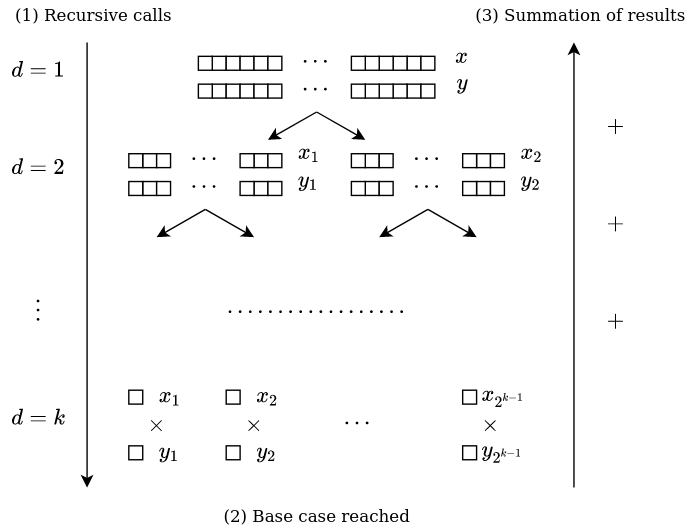
\includegraphics[width=0.7\textwidth]{images/recursive_dotprod.png}
\end{center}

Since the results of each layer are added together instead of being accumulated
into one term, error will increase after each layer of the tree, instead of
after each operation, thus growing in $O(\log n)$ as shown in \cite{higham}.

Here is the implementation of the algorithm that you can add before the main function:

\newpage

\begin{minted}{C}
float recursiveDotprod(float * x, float * y, size_t n) {
	// NOTE This implementation assumes that N can be written as 2^k
	if((n & (n - 1)) != 0) {
		return 0;
	}
	// Base case
	if(n == 1) {
		return x[0] * y[0];
	}
	// Recursive case
	else {
		// Split array in 2 and do a recursive call for each half
		return recursiveDotprod(x, y, n / 2) +
			recursiveDotprod(&(x[n/2]), &(y[n/2]), n / 2);
	}
}
\end{minted}

Call the function in \mintinline{bash}{main.c} and add a new probe:

\begin{minted}{C}
     float recursiveRes = recursiveDotprod(x, y, n);
     vfc_probe(&probes, "dotprod_test", "recursive", recursiveRes);
\end{minted}

\dots and optionally a \mintinline{C}{printf} statement:

\begin{minted}{C}
  printf("Naive dotprod = %.7f \n", naiveRes);
  printf("Recursive dotprod = %.7f \n", recursiveRes);
\end{minted}

Finally, commit and push the changes to your remote repository. Optionally, you
can also run \mintinline{bash}{vfc_ci test} yourself to generate a results file
and directly generate the report with \mintinline{bash}{vfc_ci serve} (in which case
only the results you have just generated will appear, since the first results
file is not in your work tree).


\subsection{Using the report to compare the two algorithms}

Checkout to the CI branch and launch the test report. A
second commit including the new test probe should appear. In the "Inspect run"
section, which allows to examine and compare results from a single run, we
should be able to compare the two algorithms:

\begin{figure}
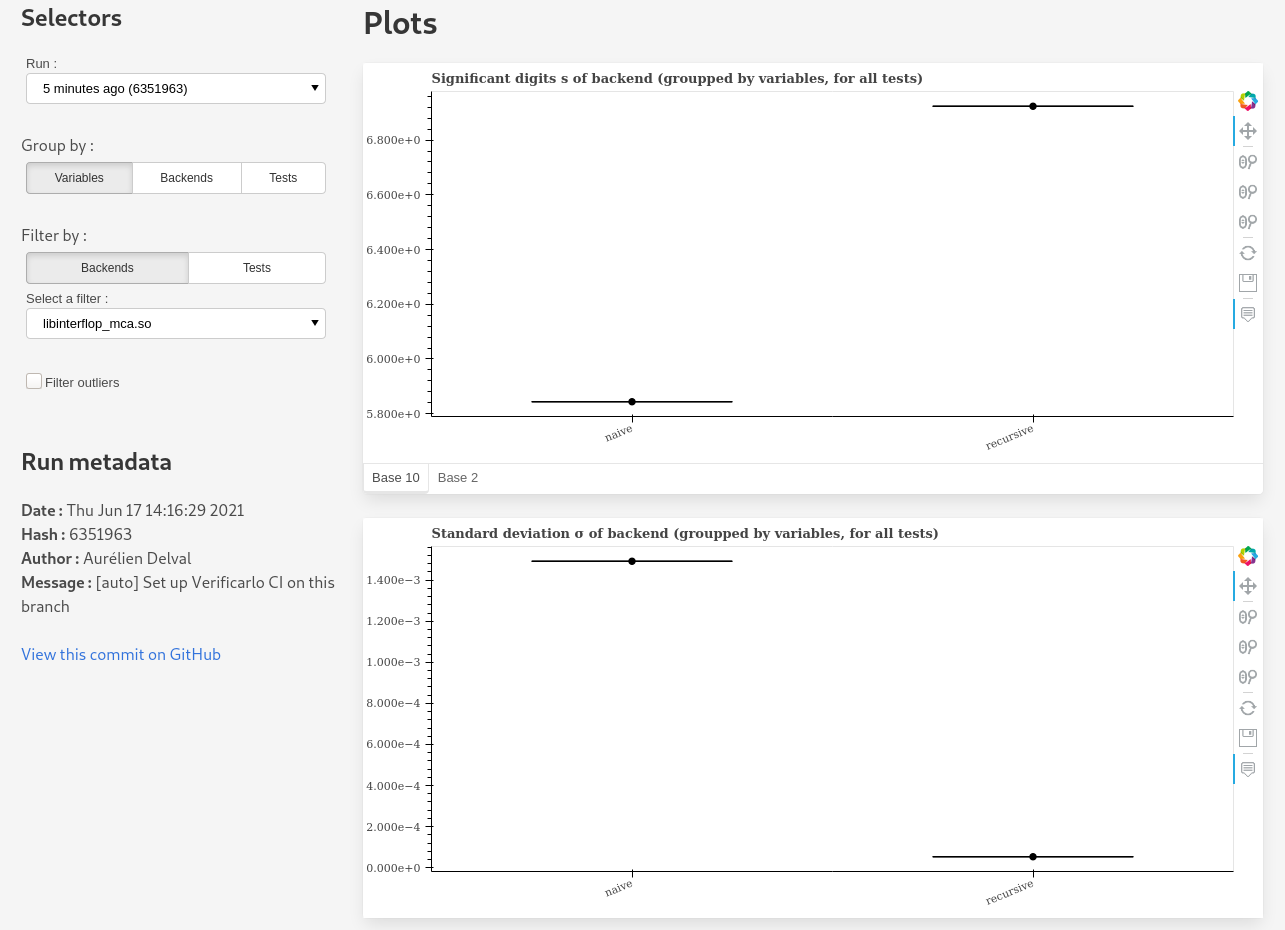
\includegraphics[width=\textwidth]{images/naive_vs_recursive.png}
\caption{Comparison of both \texttt{dotprod} algorithms}
\label{naive_vs_recursive}
\end{figure}

The following plots seem to validate our assumptions about the recursive
algorithm: the recursive version has both a higher number of significant
digits (around 6.9 vs 5.9 with \mintinline{bash}{libinterflop_mca.so}) and a
lower standard deviation with both backends.

In this simple example, \mintinline{bash}{vfc_ci} allowed us to quickly compare
two algorithms and confirm that our second one is numerically more stable than
the naive version. Of course, the proposed solution does not aim to be optimal,
and you can try to implement other methods such as the Kahan summation
\cite{kahan} or Kobbelt's dot product algorithm \cite{kobbelt}.

